\documentclass[letterpaper,twocolumn,10pt]{article}
\usepackage{usenix2019_v3}

\usepackage{amsmath}
\usepackage{graphicx}
\usepackage{subcaption}
\usepackage{balance}
\usepackage{empheq}
\usepackage[most]{tcolorbox}
\usepackage{xcolor}

\begin{document}
\title{\Large \bf OrchardScope: A Network and Computing Architecture in Precision Agriculture}


\newcommand\fatima[1]{\textcolor{magenta}{Fatima: #1}}
\newcommand\noman[1]{\textcolor{red}{Noman: #1}}

%for single author (just remove % characters)
\author{
{\rm Your N.\ Here}\\
Your Institution,
% copy the following lines to add more authors
% \and
% {\rm Name}\\
%Name Institution
} % end author




\maketitle

\begin{abstract}
There has been a huge increase in the use of data-driven techniques to help boost agricultural productivity by collecting, processing, and analyzing environmental data. In addition to farmers using more precise information about their crops, these systems can enable agriculture scientists to get more insight into factors affecting crop yields, disease detection, and pesticide spraying. However, current systems lack temporally and spatially rich data, generally assume strong cloud connectivity, and are typically non-extensible and application-specific. We present the design of \myname, an open-source and extensible system for enabling precision agriculture applications that require high resolution data and/or real-time responses. We motivate the design of our proposed system architecture through preliminary data collection efforts and a simulation study. We also highlight several system design challenges in fully deploying the system.

%There has been a huge increase in the use of Internet-of-Things, cloud or edge computing, and data-driven techniques to help boost agricultural productivity by collecting, processing, and analyzing environmental data. In addition to farmers using more precise information about their crops, these systems can enable agriculture scientists to get more insight into factors affecting crop yields, disease detection, and pesticide spraying. However, current systems lack temporally and spatially rich data, generally assume strong cloud connectivity, and are typically non-extensible and application-specific. 
%We present the design of \myname, an open-source and extensible system for enabling precision agriculture applications that require high resolution data and/or real-time response.  We also highlight several system design challenges. 

% We present the architecture, design, and preliminary evaluation of OrchardScope, a wireless sensing and computing network for monitoring plants and controlling actuating devices in the large and diverse agriculture farms. 
% The OrchardScope system consists of three tiers:  the OrchardScope node which gathers visual and environmental data, processes it, and provides a control interface to the nearby smart actuating devices, a network fabric which exposes this interface to the arbitrary network endpoints, and an application software that uses this networked interface to provide various precision agriculture applications.  
% The OrchardScope node integrates a Jetson Nano module with a high resolution camera to capture the visual data from the farm,  with optional control to attach various environmental sensors.  
% The network comprises a complete BLE stack on every node and a gateway router that connects to the external networks.   
% The application tier receives and stores readings in a cloud-based database and uses a web server for visualization. 
% Nodes join the BLE mesh network after being installed and begin interactions with the application layer. 
% We plan to evaluate our system in a preliminary deployment at a greenhouse as well as a research orchard managed by the agriculture school at a major university with 10 nodes spread over few blocks of orchard and present visual data from this preliminary deployment.
% \textbf{will update at the end.}
\end{abstract}

\section{Introduction}
\textbf{This section should not be more than 2 columns.}

The world food demand is expected to double by the year 2050, primarily driven by the upward social mobility and the increase in the world population~\cite{godfray2010food}. 
The additional problems of climate change, water shortage, and reduced agricultural land are making the problem of meeting this increased demand significantly difficult. 
It is estimated that data-driven agriculture practices can help increase the productivity of the farms by 67\% bu cutting down the losses by 2050. 
There have been very successful field trials which show that varying the water input across different places on the farm based on the sensor measurements can increase farm productivity by as much as 45\% while reducing the water intake by 35\%~\cite{almarshadi2011effects}.  Similar techniques have proved to be very beneficial to other farm inputs like soil nutrients and seeds~\cite{kim2009soil}. While there has been a lot of work by big R\&D companies such as Microsoft Research and many startups on developing smart agricultural applications for the end farmers, these efforts are highly dedicated and there is a lack of open-source frameworks that enable multiple precision agriculture applications.
\fatima{Only commercial efforts are not enough, infact academic input from agricultural and engineering experts is needed to better research the optimal use of technology in precision agriculture. It is imperative for academic community to produce open source hardware/software testbeds around precision agriculture to promote academic research.}

In addition to increasing the yields for the farmers, agriculture researchers are another potential group that can benefit from this boom in precision agriculture. The agriculture researchers may need a more in-depth insight into the farm, requiring visual and environmental data at a temporal and spatial resolution that may not be needed by the end farmers. 
The current weather models used for agriculture are very coarse and do not take into account the micro-climates that may exist within the farm. \fatima{Its better to have references for all of these claims. What damage do micro climates and pests do etc. Ask Paul for these references} There is a need to gather environmental data at a much higher spatial and temporal resolution inside the tree canopy. In addition, the prior work suggests that the pest attacks and spread of diseases can be identified by analyzing the tree leaves. However, the state of the art in this domain is to analyze the infected tree leaves manually, which does not lead to a robust response. This calls for an automated system of capturing images periodically and processing them to analyze the disease spread and pest attack patterns. The agricultural scientists are also interested in finding the correlation between the environmental variables and the diseases, an analysis that is not possible without high resolution environmental and image data.

The field of precision agriculture is in its infancy, relative to Internet-of-Things (IoT) and Wireless Sensor Networks (WSN). The precision agriculture shares many goals and constraints of IoT and WSN, such as resource-constrained devices, in the wild deployments, and need for ubiquity. The research work on precision agriculture has borrowed heavily from prior work on WSN and IoT, as summarized by Thakur et al~\cite{thakur2019applicability}. FarmBeats is the most well-known IoT platform for data-driven agriculture~\cite{vasisht2017farmbeats, kapetanovic2017experiences, jain2019low}. It shares the high level goals of our project for monitoring the farm and having processing capabilities at the edge, but it is not salable and does not allow the implementation of generic precision agriculture applications. 
Our goal is to build an interactive, near real-time, and extensible framework that monitors the smallest component in the farm i.e. leaves, as well as the fewer large trees, so that the agriculture scientists can use this rich temporal and spatial data to understand the impact of micro-climates as well as enable different precision agriculture applications.

In this paper, we present OrchardScope, a network and computing architecture for precision agriculture, that seamlessly enables different applications with very different data requirements, computation needs, and allowing different times to react. OrchardScope can ensure system availability  even  in  the  face  of  power  and  Internet  outages caused by bad weather, a fairly common scenario for a farm.  Further, OrchardScope enables cloud connectivity for the sensor data for user access and to enable persistent storage as well as long-term or cross-farm analytics. We plan to deploy our system on a green house managed by a research university as well as a research orchard managed by the agriculture department in northeast United States. At the start, we plan to enable three applications for the researchers: monitoring experiments in the greenhouse, automating apple cluster thinning task for apple orchard, and gathering large-scale visual data for disease detection. In designing OrchardScope, we solve three key challenges. 

First, to enable gathering of high resolution visual and environmental data, we design a mesh network of resourceful devices called OrchardScope nodes that are spread throughout the farm. The camera and other sensors directly connect with the node. There is a lack of power on the farm and these devices are powered by the solar panels with a battery backup. As solar power is impacted by the weather significantly, there has been some work on developing weather-aware edge devices that modulate their operations based on the weather forecasts~\cite{vasisht2017farmbeats}. However, the prior work uses outdated and inaccurate forecasting techniques. We plan to leverage recent work on developing probabilistic weather forecasts that give a distribution solar power based on the weather forecast. The probabilistic forecast approach help understand the uncertainty in the forecast value and accounting that in the operation of the OrchardScope node helps make the system more reliable. 

Second,  Internet  connection  to  the  farm  is  typically weak or in some cases non-existent making it challenging to ship high bandwidth visual data collected from the OrchardScope nodes to the cloud for processing. 
To counter this problem, we design our system with an assumption that there is no Internet connectivity to the farm in the form of high-speed internet connection from Internet providers. This constraint pushes our design towards edge computing where we equip the OrchardScope nodes with the embedded devices capable of running computer vision and machine learning tasks. We also enable collaborative edge computing for the cases where a single device will not be able to satisfy the processing needs of a particular application. We send high level summaries and data to the cloud where the researchers and farmers can get access to the data. We are also considering providing access to the data within the farm, if needed. 

Finally, while drones are one of the most exciting farm sensors today, they suffer from poor battery life. Getting aerial imagery for a farm requires multiple drone flights and a long wait time in between when the batteries are being charged. These characteristics are not suitable for our intended applications where we may need data of various parts of a single tree every few minutes, i.e. capturing multiple apple clusters on a single tree every 20 minutes. Therefore, we decide on the static placement of cameras inside the farm where each camera captures multiple trees and provides high resolution images of very tiny parts of the trees.\fatima{I think we should not highlight static placement because we have the capability of rotation and zooming in on a particular event of interest.} Our cameras use computer vision and image processing techniques to enable capturing of very small parts of the tree or get wide views that may be needed for some applications. 
\fatima{Comment on the cost of your test bed.}

% The rest of the paper is organized as follows. We describe the high level architecture of the OrchardScope in Section~\ref{fig:architecture}. The design details for the OrchardScope node are given in Section~\ref{node}, while the network details are outlined in Section~\ref{network}. The application tier is described in the Section~\ref{application}. Finally, we will present our deployment details in Section~\ref{deployments}. 
% \fatima{We can remove this paragraph.}

\fatima{It's good to write it in context of an architecture that caters to various precision agriculture applications and is extensible in terms of it's sensing, network, and compute capability to support future applications}

\section{Motivation}
There has been a lot of work on developing precision agriculture systems, both in industry and academia. 
However, it is generally application-specific, assumes internet connectivity, does not provide high spatial and temporal resolution data, and does not support real-time applications. 
In this section, we highlight the problems and how they motivate our system. 


\noindent
\textbf{Lacks high temporal and spatial resolution data:}
The existing systems focus on the use of static cameras and drones. 
The problem with static cameras is that they provide only high level monitoring of the farm. The resolution provided by them is not suitable for a lot of applications such as disease detection and pesticide spray. The drones typically have high resolution cameras and can gather data for such applications. However, management of drones fleet for high spatial resolution (images of tree leaves and individual fruits) and high temporal resolution (every few minutes) presents a significant challenge. Also, some of the applications may require that the images over time are always taken from a fixed angle, this will also be a significant hurdle for systems that only use drones and may require additional infrastructure i.e. QR tags. 
In short, the existing systems are not capable of handling scenarios where we need very high temporal and spatial resolution data with application-specific requirements. 

\noindent
\textbf{Strong Cloud Dependency:}
We should motivate against total cloud dependency by citing lack of connectivity and cloud costs. There may be places where the farmers may have internet connectivity on the farm, a system designed without this assumption would certainly be preferable. 
Second, buying a computer to do machine-learning and computer vision tasks is currently cheaper than the cloud-based options. The biggest attraction of the cloud is its scalability. 
We should present some calculations here to backup this claim. 
We should acknowledge that the training on edge devices is a challenge, but there is a lot of work on federated machine learning. 

Another point that we need to handle is the availability of the raw data and processed output to the end-user. For a farmer, they may only be interested in the final output, but agricultural scientists may also need access to the raw data. Our default setting is to process everything at the edge and give only final output. We need to address how to provide access to the raw data. We have the gateway node that connects with the cloud, but is cellular connection suitable for transferring large image data?

\noindent
\textbf{Application specific, non-extensible system design:}
Most of the precision agriculture systems that exist today cater to only specific applications. For example, See \& Spray technology by Blue River focuses only on smart herbicide spraying~\cite{see&spray}, CropX platform is designed for smart irrigation and fertilizing~\cite{cropx}, and FieldAgent and PrecisionHawk systems focus on generating field maps to monitor crop growth and health~\cite{precisionhawk, fieldagent-sentera}. The cost and complexity of combining these systems to provide an holistic view of the farms will deter farmers and academic researchers. 


\noindent
\textbf{Lack of real-time support:}

% \fatima{Another point could be that we provide an extensible test bed that can be tailored towards the needs of agriculture researchers in various domains ranging from increasing yields, sustainability, and lesser use of chemicals etc. Other solutions only cater to specific use cases?}

% \textbf{Key points on how our system is different from FarmBeats. Our temporal, spatial resolution requirements and application-specific constraints mean that drones are not suitable. Their cameras are basic PTZ cameras and they do not consider the explicit optical zoom cameras. Their network and edge-computing architecture is not suitable for a lot of scenarios.}

\section{OrchardScope Design}
% \noman{This section should start with talking about the high level goals of our system.}
% The overall design of the OrchardScope system is shown in Figure~\ref{fig:architecture}.  
% The design decomposition is three tiers: the end nodes, the network, and the server-hosted, application-specific code. 
% We outline the details of each layer next. 
% The OrchardScope node supports a set of operations such as take images, run an image processing task, and communicate with nearby actuating device . The OrchardScope network is a wireless Bluetooth Low Energy (BLE) mesh network that uses a LTE-enabled gateway to route packets between the OrchardScope nodes and other networks. The application tier consist of precision agriculture applications that interacts with the network of OrchardScope nodes via its API.

To motivate the design of our system, we present two high level requirements that meet the needs for a diverse set of emerging precision agriculture applications: 

\noindent\textbf{Temporally and Spatially Rich Sensor Data:} Agricultural scientists have long outlined the need for high temporal and spatial resolution visual and environmental data to study the existence of microclimates, the impact of microclimates on crop yields, the correlation between visual and environmental data, and the growth/spread of diseases\cite{microclimate-specifics, microcolimate-effect, microclimates}. 
    
\noindent\textbf{Low latency inference and response:} A large number of applications require near-real time response for the optimal performance, i.e. smart spraying, early disease identification, and pest attack detection. 

To fulfill these requirements, we present a three-tiered edge computing architecture: (1) The bottom-tier consists of densely deployed resource-constrained devices providing high spatial coverage. These devices are batteryless; they collect and transmit data intermittently and opportunistically. (2) The mid-tier comprises devices capable of capturing and processing high-resolution data such as video streams. It is also responsible for powering up bottom-tier devices and reading data from them. (3) The top-tier is a cloud component connected to mid-tier through unreliable network, as is the case in most farm settings. This tier has excess storage and compute capability at the cost of high access latency.

\begin{figure}[t]
\centering
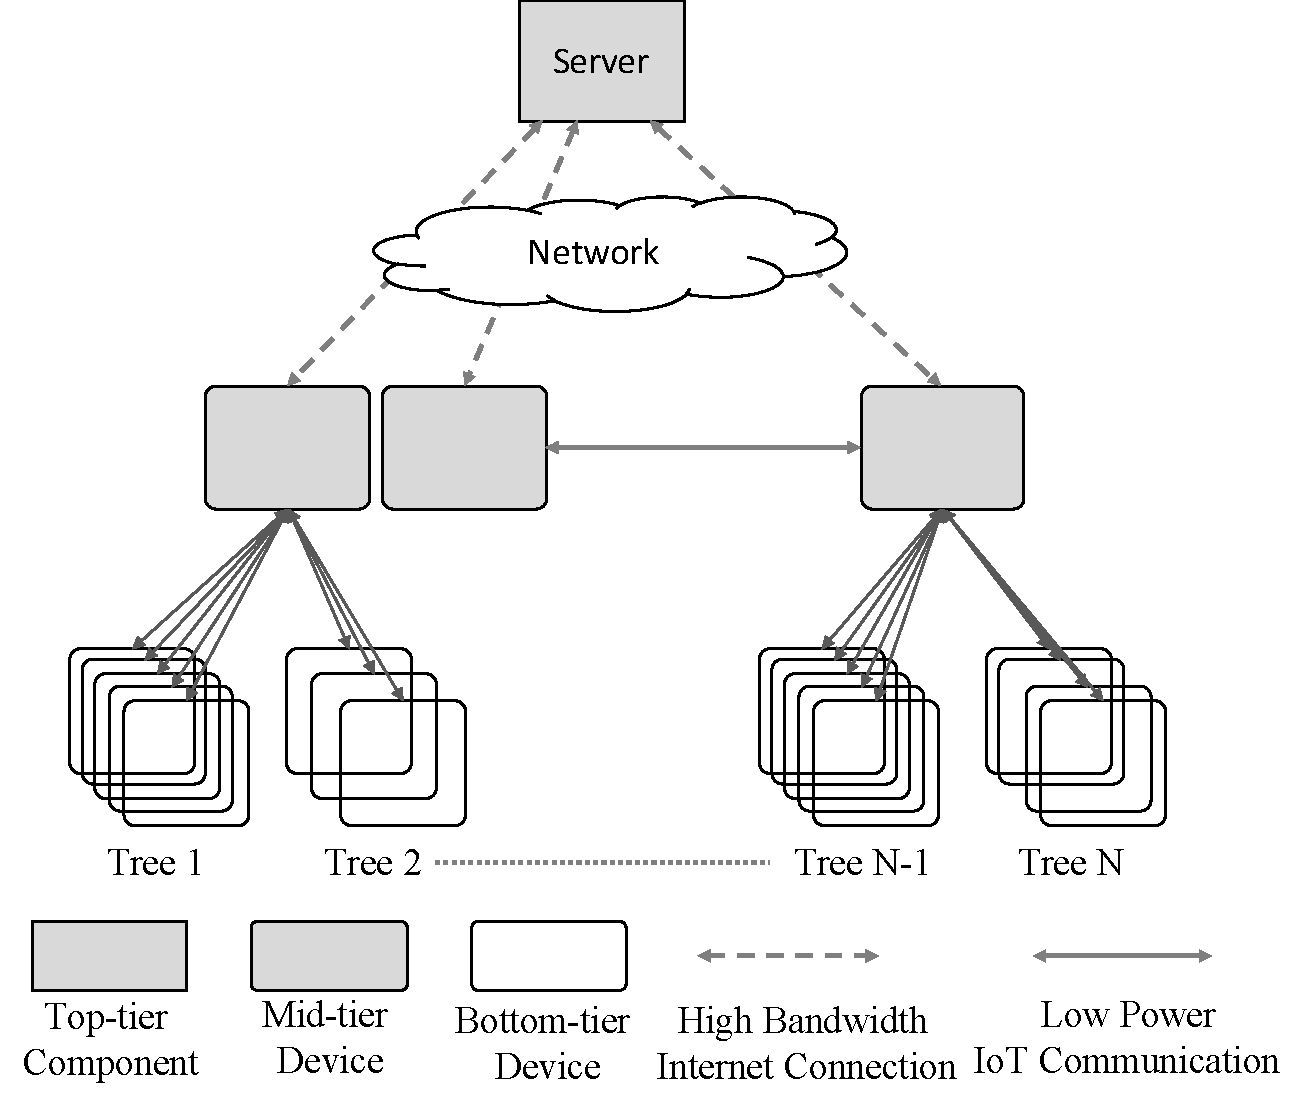
\includegraphics[width=0.4\textwidth]{./figures/arch_v2.pdf}
% \vspace{-0.4cm}
\caption{Three-tiered architecture}
% \vspace{-0.3cm}
\label{fig:architecture}
\end{figure}


\subsection{Bottom-Tier}
The bottom-tier consists of tiny, batteryless, and intermittently-powered devices that collect environmental variables such as humidity, temperature, pH, or moisture \cite{SensorsA98:online}. These sensors are based on RFID technology and implement the EPC Gen 2 protocol\cite{EPCUHFGe31:online} for communication with commodity readers. The small form factor of these sensors allow them to be deeply embedded within an agricultural ecosystem. %For example, in an orchard, there could be tens of devices per tree or  that collect data from different parts of the tree, i.e. leaves, stem, top of canopy, and roots; 
For example, in a field there could be sensors deployed on the leaves, growing fruits and vegetables, as well as in the top-soil. We advocate a battery-free approach towards sensing because of its low cost, small form factor, lack of required maintenance. Furthermore, eliminating chemical batteries will minimize potential health hazards introduced by sensor placement. 

\noindent\textbf{Design Considerations:} There are two primary design considerations in accommodating this tier of devices:
% Devices in bottom tier are only capable of data collection using tiny, batteryless, intermittently-powered devices.

\noindent\textbf{1. Power:} 
 Bottom-tier sensors buffer minimal amounts energy and are remotely powered by a radio frequency carrier. Recent work has demonstrated that RFID readers can be used for this purpose over long distances when used in a MIMO configuration \cite{wang2019pushing}. Our architecture employs proximate readers and antennas powered by solar harvesting and deployed near or within a field or tree block to periodically activate these sensors; these readers collaborate to increase coverage areas and provide power to specific subsets of sensors.%These dense deployments and high spatial resolution is difficult to achieve with battery-powered IoT sensors imposed by the power, size, and cost constraints [].   

\noindent\textbf{2. Communications:} 
The primary purpose of these devices is to take a measurement of the environmental variable they are intended for. Sensor values are locally stored when powered from the RF carrier and use a backscatter link to transmit these values to a mid-tier reader. The carrier emitter and receiver may operate as a single reader in a monostatic configuration or multiple devices in a bistatic configuration. The nodes in this tier can only transmit data to a mid-tier device and cannot talk to each other. %Also, nodes intermittently powered through laser beam can be used~\cite{naveed-lamp}. 

\noindent\textbf{Challenges:} There are many hardware and software level challenges in this tier, two of which are outlined below. 

\noindent\textbf{1. Placing readers and localizing sensors:}
One of the main challenge is to calibrate the distance between these tiny devices and their readers for optimal data collection. Increasing the number of antennas and reader potentially increases the communication range -- coordinating and aligning reader. In-the-wild deployment in a farm settings make these tasks more challenges as weather may impact the device characteristics; the location and orientation of devices may change over time. 
Another key challenge is to estimate how many devices can be accommodated by each reader given the device power requirement and time resolution.   
% \noindent\textbf{Determining ideal power and duration:} An important challenge is to determine how much power and for how long is required for an accurate reading. It is important to strike the right balance as higher power levels for long duration may lead to time and energy waste, while low power for short duration may result in missing or erroneous data. 

\noindent\textbf{2. Handling missing or erroneous data:}
 There is a possibility of missed or erroneous communication with intermittently powered batteryless devices and software capable of extracting knowledge from missed data needs to be explored. 


\subsection{Mid-Tier} 
The mid-tier consists of resourceful devices (i.e. cameras) that collect data from bottom-tier sensors, process and aggregate data from variety of sensors, make real-time actuation decisions, and forward the collected data to the top-tier. Mid-tier devices are placed such that they are able to both collect data from bottom-tier devices and are also able to capture diverse images from areas of interest.

% \noindent\textbf{Device Placement:} The mid-tier nodes are sparsely deployed across the farm. The placement of these devices depends upon the technology used in the bottom-tier, the resolution requirement of the video streams for apple thinning like applications, and placement of actuating devices and their communication technology. For example, RFID-based bottom-tier nodes may require the mid-tier device to be at maximum of 100ft for reliable data collection, the camera resolution may dictate a mid-tier device for each block of trees, and actuation device communication technology may need the mid-tier node to be at maximum of 50ft. The mid-tier nodes placement is such that it satisfies all the constraints. The requirement of high resolution images from a fixed angle for apple thinning application motivated the static deployment and careful placement of the mid-tier node as well.

\noindent\textbf{Mid-tier Services:}
Devices in mid-tier provide various services to enable the aforementioned applications.\\

\noindent\textbf{1. Data Collection:} The mid-tier nodes power the densely deployed battery-free bottom-tier nodes in their vicinity and receive data from them. Additionally, they themselves gather data from sensors that are directly interfaced with them, i.e. cameras, anemometers, pyranometers, wind gauges.\\
\noindent\textbf{2. Aggregation \& Inferencing:} The mid-tier nodes are responsible for aggregating data from different sources such as bottom-tier nodes and high-resolution sensors, in order to enable precision agriculture applications that require the data from multiple sensors to make inferences. %For example, microclimate analysis application needs to combine data from different environmental sensors and insecticide spraying needs temperature and visual data. 
These inference tasks are enabled by machine learning and computer vision techniques. To enable the data processing, aggregation, and inference tasks, mid-tier nodes require a processor that provides these interfaces and are able to run ML/AI tasks.%, i.e. Jetson boards, Coral Edge TPU, BeagleBone AI, Arrow I.IMX8X, etc.

% Aggregate data collected from bottom-tier devices and other mid-tier devices to make real-time inferences.
%\\\textbf{3. Forwarding:} Mid-tier nodes are capable of horizontal as well as vertical communication in both directions. In the vertical direction, they gather data from bottom-tier nodes and upload data aggregated at the mid-tier to the top-tier. Additionally, the mid-tier receives data and control instructions from the top-tier to enable precision agriculture applications. The link between these tiers will be enabled by a high bandwidth communication technology such as WiFi or cellular. Peer-to-peer communication between mid-tier nodes enables data sharing, aggregation, and collaborative edge-computing tasks using a low power wireless protocol, i.e. Bluetooth 5.0, IEEE 802.15.4. Collaborative edge computing can enable or improve the performance of applications. %For example, the apple thinning application can combine partial images of apple clusters captured by different cameras or run a computationally-intensive cluster sizing algorithm on multiple mid-tier devices. 
% For example, mid-tier devices may communicate to share the data about a tree that is partially covered by two devices or they may need to run a heavy ML/AI task across multiple devices. 
\noindent\textbf{3. Actuation:} The mid-tier nodes communicate with actuators to perform tasks based on real-time inferences. The actuation device may be directly interface through a wired or wireless protocol. The real-time processing and actuation capability is necessary for time-critical applications. 
%such as smart insecticide spraying, where the delay introduced by using cloud resources over an unreliable network will lead to disappearing of pheromones effect, poor eradication of insects, and waste of spray.

\noindent\textbf{Challenges:} The challenges at the mid-tier relate to the data collection from bottom-tier, edge computing, and energy harvesting issues. There are also challenges related to data aggregation or sensor fusion across various sensors etc. 

\noindent\textbf{1. Energy Management:} Grid power is not typically available at remote farm locations and mid-tier devices will need to harvest energy for their operations. The energy harvested from these renewable resources is highly stochastic and dependent upon weather and shading from nearby trees. The mid-tier devices will need to predict energy harvested in the future and schedule diverse activities including bottom-tier sensors, sampling mid-tier sensors, running inferences, and communicating data within and across tiers.  

% \noindent\textbf{Managing Bottom-tier Devices:} To enable high spatial resolution, bottom-tier nodes need to be deployed in large numbers in a way that does not require careful installation. The large number is needed to cover the different parts of the canopy and avoiding careful installation will enable practical deployments. In addition, these devices may move due to wind, rain, and irrigation water. The task of locating, powering, and reading data from these floating devices will present unique challenges. 
    
% \noindent\textbf{Energy Harvesting:} The grid power is typically not available in the farm and mid-tier devices will need to harvest energy for their operations from source such as solar PV, wind, etc. The energy harvested from these renewable resources is highly stochastic and dependent upon weather and shading from nearby trees. The mid-tier devices will encounter the challenge of predicting the expected energy into the future and schedule their operations based on the energy budget.  
    
\noindent\textbf{2. Collaborative Edge Computation:} Some of the mid-tier services may need collaboration across devices. For example, the microclimate analysis application needs to fuse environmental data from different locations in the farm. Collaboration among devices raises challenges related to energy management, networking, and scheduling tasks. 

\noindent\textbf{3. Developing Data Pipelines:} The mid-tier devices will be collecting a lot of high temporal and spatial resolution data about multiple variables. All the applications will not require the same or even the highest resolution. For example, microclimate analysis application will require visual data only at the time resolution of the environmental data. The mid-tier device should develop pipelines that provide the users or the applications an access to the data from the required sources at the desired granularity. 
    
    % The network connection with the top-tier can be unreliable, as in most farm settings. The network connectivity may be possible at only one or few of the devices in the mid-tier. This situation raises challenges related to data aggregation across nodes. 

% \fatima{You can replace "bottom-tier" sort of names with something relevant. Figure is only for reference. You can modify it in any way.}



\subsection{Top-tier}

The top tier is hosted in the cloud through an unreliable high bandwidth network and provides the user an interface to deploy applications, view data or application summaries, access the raw data, provides sensor measurements on-demand. 

\noindent
\textbf{Top-tier Services: } The top-tier of \myname{} provides various services that are outline below. 

\noindent
\textbf{1. Simplifed Application Deployment:} The primary task of the user is to deploy applications ranging from generic tasks of gathering particular data at a desired granularity to deploying specific applications such as smart insecticide spray. The user can specify the required data pipeline for different applications and should be able to connect the appropriate data pipeline to the input/output of the application-specific code. The top-tier provides the user with an ability to push application code, AI/ML model training jobs, or run diagnostic code. Additionally, the applications that are not latency-sensitive and require significant resources can be deployed in the cloud to save energy and computational resources at the edge.
%, i.e. For example, the output pipeline of smart insecticide spraying will connect to the actuator input to release the spray. 


\noindent
\textbf{2. Summary and Overview:} The user will be able to access the summary of the collected data or results of deployed applications. For example, user should be able to map the temperature differential across microclimates, look at the temperature profile of a tree, or inspect the post-insecticide spraying images to visualize the number and types of insects killed. 

\noindent
\textbf{3. Raw Data Access:} The user, especially academic researchers, need access to the raw data to either build new applications or retrain the existing ML applications that can not be trained across resource-constrained mid-tier devices. 

\noindent
\textbf{4. Data On-demand:} The application tier provides manual control to the academic researchers who desire the ability to control cameras and sensors to acquire data on-demand or locate new objects of interests in the farm. This access allows fast and easy labeling of new objects to be monitored and a sanity check on the sensor data or the application output. \\

\noindent\textbf{Challenges:} We next outline the challenges faced in the design and development of the \myname{} top tier.

\noindent\textbf{1. Cloud vs. Edge:} \myname{} will run all the latency-sensitive applications at the edge. For the non-time sensitive applications, the aim is to deploy those at the edge if enough computational and energy resources are available. However, estimating available resources at the edge and deciding which applications run there presents significant challenges.
    
\noindent\textbf{2. On-demand Access:} Providing manual user control while satisfying the requirements of the applications that are running on \myname{} mid-tier devices will be a challenging task. It will be interesting to see how extensive work on scheduling interactive and batch jobs on server can be applied to solve this problem~\cite{parallel-scheduling}.
    
%\noindent\textbf{Edge Training:} There has been a lot of work on training ML models across distributed edge devices~\cite{federated-ml}. However, training models on resource constrained solar-powered nodes will pose unique challenges. 
    
%\noindent\textbf{Effective User Interface:} The task of developing data pipelines, developing application code, integrating applications with data, and using on-demand access can be very challenging for users who are not expert in the field. It will raise challenges related to human computer interaction, i.e. providing easy to use interface with clear instructions. 


% \subsubsection{Performance Evaluation:} We will evaluate the system performance on the basis of average data rate achieved in the network, its packet reception rate, and the number of devices the network can support. 

% \subsection{Evaluation}
% This section outlines the proposal to perform evaluations for various aspects of the OrchardScope node. The first step would be to measure the actual power consumption of the devices under various operating conditions. The next step would be to measure the quality of DC power supply and its efficiency. The third step would be stress test the computaion engine of the node to see how much computation can it perform and how its power requirements change with the load. For the radio, we need to test the range and the data rate provided by the BLE enabled nodes. Finally, we should use solar performance modeling and forecasting to analyze the operation of the solar power supply for a typical year in various location inside United States. We plan to use Solar-TK, a black-box data-driven toolkit for solar performance modeling and forecasting for the task~\cite{bashir2019solar}. 



% \begin{figure}[t]
% \centering
% 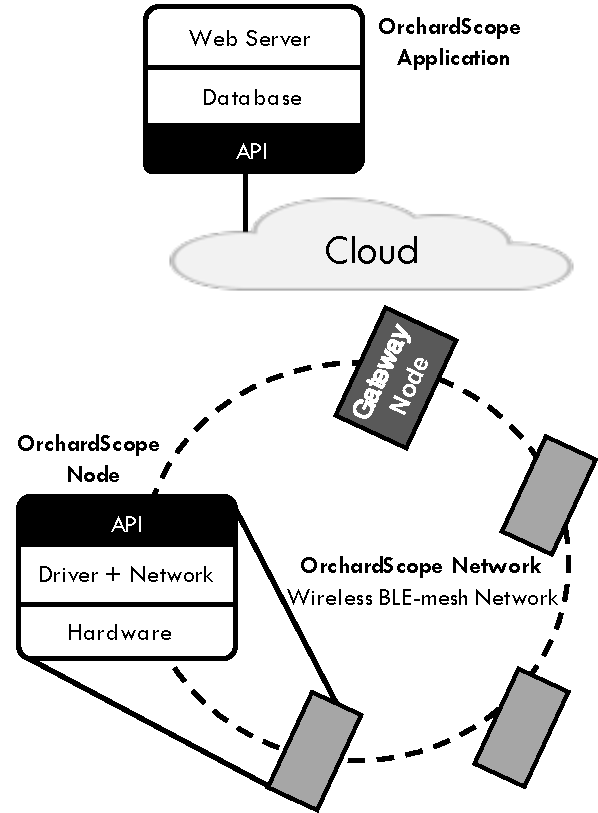
\includegraphics[width=0.4\textwidth]{./figures/architecture.pdf}
% % \vspace{-0.4cm}
% \caption{Three tier OrchardScope system.}
% % \vspace{-0.3cm}
% \label{fig:architecture}
% \end{figure}

% In the following sections, we present the design and implementation of each tier of the OrchardScope system.  At the node level, we discuss the various trade offs present in the hardware design, and present a narrow interface to access the hardware. Equally important, we consider physical design issues such as form factor and weather-proofing, which must be addressed for a deployment in an outdoor setting to be practical.  The result is the OrchardScope node:  a small form-factor device with sensing, control, and networking integrated into one package. 

% A set of disconnected monitoring devices is much less interesting than real-time data. The current wireless sensor network applications in agriculture monitoring typically use standalone designs that target one specific application, have a small LCD, a serial port, or other wired ports connecting instruments to data loggers. 
% A key motivation of our work is to allow the quick deployment and instrumentation of a large numbers of monitoring devices and enable continuous real-time access. Requiring connectivity over USB, serial, Ethernet,  or other wired channel would not be practical.  

% Finally, application specific code is placed in the cloud that is connected to the OrchardScope nodes network. Applications use the node API as exported over the network. Typically, a server daemon populates a database that is accessed by a variety of web applications, but direct access to OrchardScope using REST API is available too. We present an apple cluster thinning application which allows researchers to monitor the apple cluster over time, deploy computer vision algorithms to determine the cluster sizes, and perform the computation to determine the amount of thinning spray needed. A key architectural separation is that applications are developed independently from the network used. 


% \subsection{OrchardScope Node}

% The OrchardScope node consists of four primary components: sensors, power supply, processing unit, and a radio for OrchardScope network
% % , as shown in Figure~\ref{fig:node}
% . We next describe the choice of OrchardScope node components and how each satisfies the high-level goals of OrchardScope system. 

% % The sensor component is user-configurable where user can select which sensors are attached to the device, i.e. camera, temperature, moist, and humidity. The data from the sensing components is received by the computational engine, which processes the data using sensor-specific pre-processing techniques. The computational engine is also responsible for running the user-specified machine learning or computer vision models on the data. The power source components harvests solar energy and converts it to the appropriate DC levels required by the various components in the system. Finally, the radio is used to communicate with other devices in the network. While most of the devices in the network will have the aforementioned four components, the gateway devices in the network will have additional radios that will allow internet connectivity. 

% % There are several design choices for each component, each with its own advantages and disadvantages.  Design  decisions  for  the  different  components  of OrchardScope are not independent.  For example, a particular choice of internet connectivity enabling technology  will dictate how much computational power we have at the edge. We find that there are only a few internally consistent combinations, each appropriate for a distinct class of applications. To fully explore the available design space we plan to build two types of nodes, one for monitoring in-door spaces such as greenhouses with grid connection and WiFi connectivity available, and the other for the outdoor spaces without any power source and internet connectivity.  We plan to compare the two designs and evaluate their effectiveness for our application in future.

% % \begin{figure*}[t]
% % 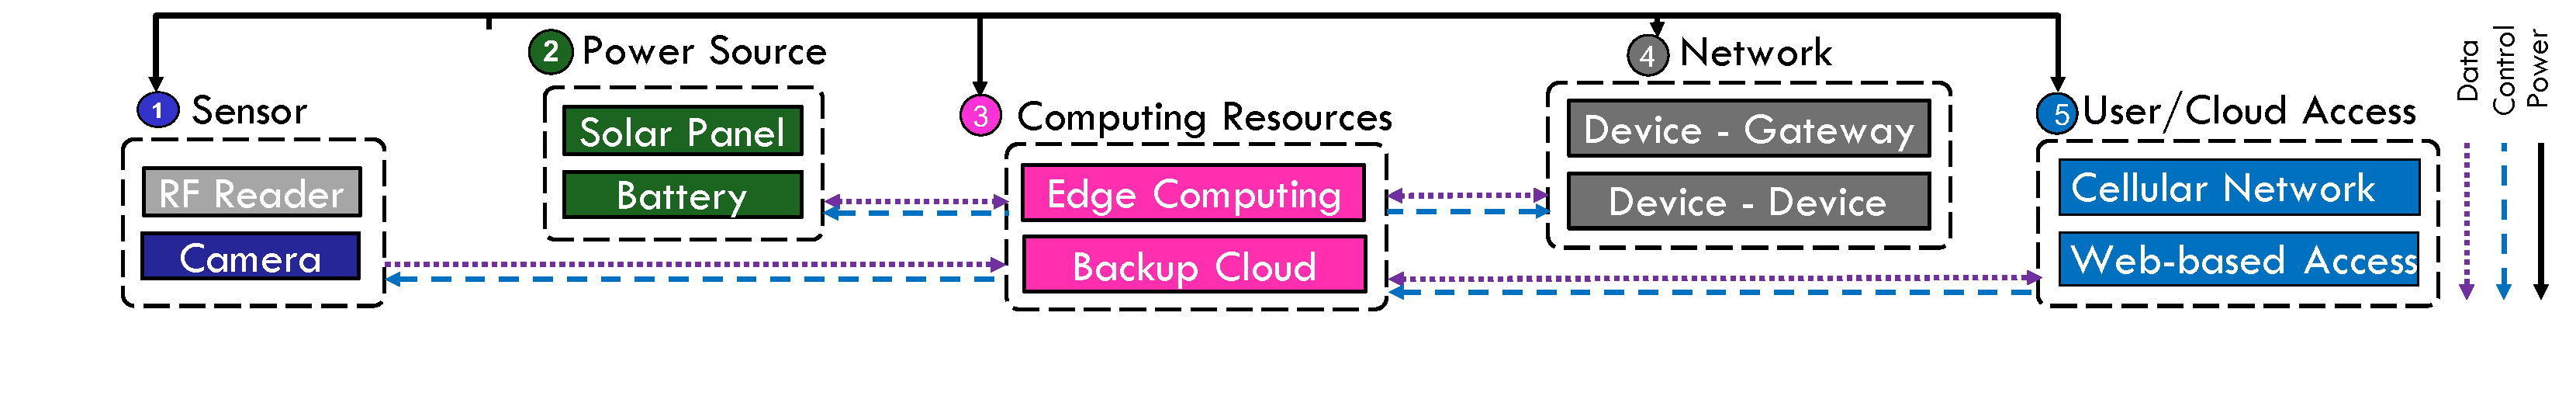
\includegraphics[width=\textwidth]{./figures/node.pdf}
% % % \vspace{-0.4cm}
% % \caption{OrchardScope consists  of  five  primary  components:   sensors, DC power supply, computational engine, a radio for OrchardScope network, and an optional radio for internet connectivity.}
% % % \vspace{-0.3cm}
% % \label{fig:node}
% % \end{figure*}

% \noindent
% \textbf{A. Sensors:}
% \label{sec: sensors}
% Two types of sensors are connected to the OrchardScope node: cameras directly connected to the node and environmental sensors interfaced using RFID reader.

% % There are multiple sensors that can be used to measure various aspects of agriculture, i.e. humidity, temperature, soil moist level, and wind speed sensors. However, while designing the OrchardScope, we are primarily interested in deploying a camera to enable computer vision based precision agriculture applications. We evaluate the difference and trade-offs between various architecture to provide visual coverage of the farm based on the extent of coverage provided and cost incurred. 

% \noindent
% \textit{\textbf{Cameras.}}
% The goal of the cameras is to take high resolution images of the different entities inside the farm, i.e. tree leaves, leaf stems,  fruits, insect traps, and ground under the trees. To meet these requirements, we use a variable focal length high resolution camera with pan-tilt-zoom (PTZ) capabilities. The focal length of the camera is chosen such that it is able to take the image at the required resolution (i.e. 1080p) of the desired object (i.e. leaves 5inx5in) at a distance (i.e. 30ft). Simultaneously, it should have a wide view to capture low resolution wide images for the applications that do not need high resolution, i.e. counting dropped fruits on the ground. 

% % Focus on design as drones have already been discussed in motivation section.

% % points
% % Drones are not good. 
% % Static cameras either do not provide high resolution or very high resolution cameras are very expensive. 
% % The solution is the variable focal length high resolution camera. 
% % It provides high resolution images of the farm at various scales. 

% % Drones are the most commonly visual sensing equipment used for mapping the fields and farms in various precision agriculture applications. However, drones are not suitable for applications where you need visual data at high temporal resolution, require high resolution images of small parts of the farm i.e. tree leaves, and have 

% % They are suitable for applications where the temporal resolution of visual data captured is low. However, if the images are required more frequently, the drones may not be a suitable option as it would not give the drones enough time to recharge the batteries. It would be an option to increase the size of drone fleet, but it would incur additional costs and operating a large fleet would be complex. In addition, the drones may require FAA approval for their operation.  

% % Most of the precision agriculture application that we consider need images of tree leaves and fruits, i.e. apples in case of an apple orchard. Given this scenario, one option was to install a low resolution cameras on the tree branches and very near to the subject that needs to be captured. This option allows us to use low-cost, low resolution cameras and still get high enough resolution required for our tasks. However, installing devices on tree branches will require careful human labour-intensive installation and maintenance. In addition, the devices may get damage during the spraying or other invasive tasks on the tree. 

% % The other end of the spectrum is to install a single, high resolution camera with telephoto lens on top of a pole in the middle of the farm. In this case, the camera is capable of taking wide pictures of the farm and has the ability to zoom into specific parts of the tree to take pictures of apple clusters and leaves, if needed. This design choice offers easy installation and maintenance. However, the key problem with this choice is the cost and the single point of failure. The cost per unit area of very high resolution cameras ends up being much higher than any of the other options we consider. In addition, installing a very expensive single camera is not practical in the sense that the data will not be collected if it goes down and also the cost to replace it would mean building almost everything from scratch again.  

% % A moderate option would be to install mid-resolution cameras distributed throughout the park that monitor only a couple of trees that are nearby. This option lies between the option 2 and option 3 in terms of cost and complexity of installation and maintenance. We have decided on using a static focal length camera without the zoom capability, as we determined that the cameras with the programmable zoom capability were significantly expensive than those of static focal length. Therefore, instead of zooming into different places, we plan to take images with a fixed zoom and adjust the distortion in the software. This setup also requires a pan-tilt assembly that allows the camera to capture multiple trees. Also, the devices containing cameras would connect with each other using a mesh network and be able to share the data they gather. 

% % The choice of camera is dictated by three factors: the size of the object to be captured, the distance of the object from the camera and the required resolution for the image. A typical apple cluster is 12in x 12in, it is at a 15-20ft distance from the camera, and we would like to capture the image at 1080p atleast. Given these specifications, we can use the arc length formula to compute the field of view for the camera. If the radius is r, and the internal angle is $\theta$, the arc length is L is given by $r\times \theta$. We can compute the internal angle required from this equation, which comes out to be $\sim 5.4^o$ for a 1080p resolution camera or $~\sim 21.6^o$ for a 4K camera. The relationship between the field of view (FOV) and the focal length is given by the following equation. 

% % \[FOV = 2 \times arctan (x / (2 f)) \]

% % Here, f is the focal length and the x is the diagnol of the area that we are trying to capture. Using this formula, the focal length required for the 4K camera comes out to be around 113mm. 

% \noindent
% \textbf{\textit{Passive RFID Sensors for Environmental Variables.}} Our system monitors the different environmental variables, i.e. temperature, humidity, using low-cost RFID-based sensors that are densely deployed across the farm. The sensors are passive and need to be powered by an RFID reader when the measurement is to be taken. The RFID reader integrates with the OrchardScope node and is controlled by the OrchardScope application to gather data at the desired time granularity. The details on the design of the sensors, their deployment, and data collection mechanism are outside the scope of this paper. 

% % \fatima{Have a single subsection on cameras and also talk about RFID tags on leaves and how you need a reader at the edge too.}

% \noindent
% \textbf{B. Power Supply:}
% The OrchardScope node will typically be deployed in the wild, where the power grid is not available. Our design uses solar power coupled with a battery-backup to power the OrchardScope node. The size of the solar panels and batteries is dictated by the power requirement of different OrchardNode components, the resource requirements of OrchardScope applications, and the days of autonomy desired for places which observe extreme weather conditions such as snow storms. Therefore, the sizing of solar + battery backup is an implementation-specific and we use an approach outlined in [cite] to determine the actual size of panels and batteries. 

% The different components of the OrchardScope node may have different voltage requirements, i.e. embedded devices typically require 5VDC while cameras may need 12-24VDC. Therefore, we use DC-DC converters to provide 5V and 24V, in addition to the 12V battery outlet, as all of the OrchardScope node components operate on one of these voltages. 

% % In such scenarios, wireless sensor networks rely on either using batteries or harvesting energy available in the environment. The batteries are not ideal for our energy-intensive devices as we require data collection and processing at high temporal resolution. Solar panels coupled with a battery backup for night time operation are the most popular choice now a days. We next present the design of our solar + battery backup. 

% % \textbf{Solar + Battery System Design:} The sizing of solar panels and batteries for specific energy needs is a well-studied problem. The first step in this process is to estimate the net energy requirement for the system. In OrchardScope, the major components that consume energy are the Jetson Nano board, camera pan-tilt assembly, camera, and radio. The power requirements and the daily energy requirement for each of the components is listed in the Table~\ref{tab:energy_requirement}.

% % \begin{table}[]
% % \begin{tabular}{|l|l|l|}
% % \hline
% % \textbf{Component} & \textbf{Power (W)} & \textbf{Energy (Wh/day)} \\ \hline
% % Jetson Nano        & 10                 & 60 @ 20minutes/hour                \\ \hline
% % Camera             & \textless 5        & 30 @ 20minutes/hour                \\ \hline
% % Pan-tilt assembly  & \textless 5        & 30 @ 20 minutes/hour               \\ \hline
% % Radio              & negligible         & negligible                         \\ \hline
% % Misc               & variable           & 30                                 \\ \hline
% % Total              & $\sim$35           & 150                                \\ \hline
% % \end{tabular}
% % \caption{Power requirement and energy consumption of various components}
% % \label{tab:energy_requirement}
% % \end{table}

% % The average energy requirement for the whole system is $\sim$150Wh. However, solar power is highly dependent on weather and in some places, i.e. northeast USA, there may not be any solar generation following a snow event. 
% % Therefore, we would like to have some backup energy stored in the battery for the days when there is no generation. We pick 3 days of autonomy for our system, which means that the total energy to be stored in the battery backup should be $(1+3) days\times 150Wh/day = 600Wh$. The size of the battery to store 600Wh at 12V should be 50Ah. Assuming 50\% depth of discharge, the lowest state of charge allowed, the battery size should be 100Ah in order to ensure longer life for the battery. The next task is to decide on the size of the solar panel such that the energy generated in a day should be 600Wh. We can assume the average day light hours to be 8hrs for most of the places in the United States. This setup means that the size of the solar panel should be $600Wh/8h = 75W$. However, the solar panel would not always produce 75W for all 8hrs of the day. Therefore, we need to pick a slightly bigger panel size of $\sim$100W. 

% % We have sized the solar panel and the battery backup for the energy requirement that we have chosen. However, this systematic approach can be used for sizing the solar panel and the battery backup for any energy requirements. 

% % \textbf{DC Power Supply Design:} We design our power supply as online backup where solar panel charges the battery and all the components are connected to the battery. This ensures that the short fluctuations in the solar power do not effect the power quality of the DC power supply. While the battery voltage is 12V, the different system components may not operate at the 12V, i.e. Jetson Nano requires 5V power supply while pan-tilt assemply needs a 12V power supply. Therefore, we design our system to provide all the different voltage levels required by the different components, which in this case are 12V and 5V. We can get the 12V directly from the battery, but a DC-DC converter is required to step-down the voltage level from 12V to 5V. The design of an efficient DC-DC converter is outside the scope of this paper and we simply use a DC-DC converter IC for this task. 

% \noindent
% \textbf{C. Processing Unit:}
% OrchardScope node uses Jetson Nano~\cite{jetson-nano} as its main processing unit because it offers a low-cost solution to run multiple machine learning applications in parallel while enabling easy interface of variety of sensors, i.e. cameras through CSI or ethernet interface, RFID reader using xyz. 
% The small size and low-power requirement make it suitable for in-the-wild and low energy applications. The computing power at the edge provided by Jetson nano allow us to enable applications that require real-time response even in the presence of low/intermitten Internet connectivity. 

% % There are four key tasks that will be performed at the OrchardScope node. The first task is the collection of data from the sensors. The second task is to clean the data and prepare it for various applications. The third task is to perform application specific tasks on data i.e. running a computer vision or image processing model to determine the attack of a pest. The final task is to make the findings available to the end user. 

% % One of the key goals of OrchardScope is to provide real-time feedback required for some precision agriculture applications. 



% % The first task of data collection needs to happen at the end device, while the other tasks can be done at the edge device or the data can be sent to the cloud where all processing is done. The cloud option is attractive as it provides infinite capacity and is cost-effective due to intense competition among cloud providers. However, it has two major drawbacks. The first drawback is that sending all the data to the cloud and back would generate a lot of data traffic. This is generally not a problem for WiFi networks, but it would be incur very high costs for scenarios where internet connectivity to the farm is established only using LTE technology. It would also incur high network and storage costs from the cloud provider. In addition to this, the second drawback is that the cloud-based computation will not be able to support real-time applications that researchers or farmers may want to deploy. 

% % Considering our choice of network and the cost of a cloud-based option, we have decided to put enough processing at the edge to enable real-time applications and use the cloud to only provide the user interface. We use Jetson Nano as the primary processing unit as it offers the general purpose IO ports (GPIO) for sensor interfacing as well as enables various machine learning model deployments. It is a small, powerful computer that lets you run multiple neural networks in parallel for applications like image classification, object detection, segmentation, and speech processing. Another attractive feature for the Jetson Nano is its very low power consumption of around 10W at its maximum use. 

% % In our setup, the Jetson Nano is responsible for collecting data from the sensors using different interfaces, i.e. USB for camera, I2C to control pan-tilt assembly. It then processes the collected images for different applications i.e. concatenates the smaller images at high resolution to generate bigger images that may be required for some other applications. Finally, it runs the user-specified machine learning tasks on the collected visual data, i.e. using computer vision to determine the size of the apples in the clusters. The final task of providing user access is done through the cloud as this OrchardScope edge network may not be available all the times. 

% \noindent
% \textbf{D. Radio:}
% The next key component is the radio that we use for the communication between the devices and the device's connectivity to the internet. OrchardScope node uses Bluetooth Low Energy (BLE) radio to communicate with its peers due to its low cost, low power, and inherent support for mesh networking. BLE 5.0 offers data rates upto 5Mbps, which enable collaborative edge applications. OrchardScope uses a gateway node that gathers data from the orchardscope nodes to send to the cloud and also receive application code from the cloud that is deployed across the network. We use cellular network to provide the edge-cloud connectivity due to its ubiquity and high data rate. A third radio on the gateway device is that enables high bandwidth link between the gateway and the moving vehicle that collects raw data. \noman{needs discussion.}
% % Both communication tasks present different challenges and we decided to use different communication technologies for each, the choice and properties for each network are described next. 

% % \noindent
% % \textit{\textbf{OrchardScope Network.}} This is the network that exists between the OrchardScope nodes deployed at the edge. The key requirement for the communication technology for this part of the network was that it is low cost, low power, and offers support for mesh networking. The WiFi was an option, but its relatively higher cost and high power requirement made it unsuitable for the task. 802.15.4 based protocols/technologies i.e. ZigBee offered low power and low cost, but the maximum data rate of $\sim$250kbps was very low for some of the collaborative edge applications we envisioned. Therefore, we decided to use the Bluetooth Low Energy (BLE) mesh network as it provides inherent support for mesh networks, is low cost, low power, and its 5.0 specifications support data rates upto 2Mbps. We have decided to use nRF52 BLE development kit for our prototype, which supports BLE mesh network. 

% % \noindent
% % \textit{\textbf{OrchardScope Cloud Connectivity.}} The second aspect of the network design was to provide cloud connectivity to the devices and allow user to access the data. The devices use BLE mesh network to communicate with each other, we decided to use LTE to connect the devices to the internet. One option was to equip each device with LTE, but this would have increased the cost of each device. The other extreme was to have a single gateway device in the network that gathers data from all the devices and connects to the internet. We decided to use a moderate scheme where gateway devices are spread throughout the network to provide redundancy for the connectivity and also enable the high data traffic that may be needed to upload high resolution video data to the cloud. We plan to investigates the LTE capability and which specific module is to be used. 

% \noindent
% \textbf{E. Node Software:} 
% The OrchardScope node needs to implement some functionality in the software to enable some of the applications. The first key task is the acquisition of visual and environmental data by controlling camera and RFID reader, respectively. The camera control strategy decides on which object to capture, when to capture, and the desired resolution of the object of interest. Similarly, RFID reader control decides on which passive sensors to power, the time duration and strength of power, and how often the data should be collected. The next task is to process the collected data and prepare it for OrchardScope applications as well as sharing with the end user, i.e. concatenating partial images collected from different cameras. The third task is to run the machine learning and computer vision models that the user may have deployed as a part of OrchardScope application. Lastly, the node needs to manage its energy budget by forecasting solar power and estimating the energy requirement of different tasks, i.e data acquisition and running ML models. 


% % \noindent
% % \textit{\textbf{Camera Control.}} As discussed in Section~\ref{sec: sensors}, we have decided to use a mid-resolution camera mounted on a pan-tilt assembly that covers multiple trees. In order to enable that, we needed to design a camera control strategy where we decide on how we move camera to capture all the different parts of the trees under observation. There are two important factors that govern this decision: the distance of the tree under observation from the camera and the minimum resolution of the pan-tilt assembly. In our example deployment case, the distance between the camera and the tree ranges from 15ft-20ft. The minimum resolution provided by the pan-tilt assembly is $0.29^o$. A movement of $0.29^o$ by the pan-tilt assembly will shift a distance of 0.91in and 1.21in at 15ft and 20ft, respectively. The distance is approximately computed by the following formula. 

% % \[ arc\ length = radius \times central\ angle \]

% % This resolution is high enough to capture the smallest parts of the tree. However, as it is evident, the distance moved by a fixed degree movement by the assembly depends upon the distance of the tree from the camera. Therefore, we will need to adjust the angle moved in order to get the consistent coverage of the trees under observation. In our current implementation, our camera control algorithm simply divides the area under observation into a grid where it moves along the rows from left-right (for odd rows) and right-left (for even rows). This approach is simplistic but has two key drawbacks. First, we may be interested in capture only a particular part of the trees and we would need to reconstruct the whole image from these small parts and then find the desired image from the bigger picture. Secondly, the individual pictures along may not capture the desired object fully, i.e. an apple cluster that we want to capture may be divided in two cells. This would also require generating a bigger picture from the parts and locating apple clusters. However, this reconstruction will incur some losses and the desired object may be deformed. 

% % We are considering using computer vision techniques to identify where the images need to be taken. For example, in case of capturing apple clusters, the camera will scan the apple tree and the video stream would be processed by a computer vision model which will save the image only if it captures the object under consideration. However, this requires pre-training of the models to detect the desired objects. The acquisition of data for the training and training may not be very straightforward. 

% % \noindent
% % \textit{\textbf{Image Concatenation.}}
% % The mid-reolution camera only captures a 1080p images of a 5in$\times$5in image. However, for some of the applications, the researcher may require a bigger image and the smaller images may need to be concatenated. We currently implement a very simple image concatenation technique which uses Python Pillow library to stack images together. However, this assumes that all the images do not overlap and the do not have distortion. These assumption may not hold true in practice as imprecise movement of pan-tilt assembly would result in some overlap or some parts of the images missing. Also, the pictures will be taken at different distances from the camera, which means the size of the images and the angle at which the image is taken will be different. There is a need for a better concatenation techniques that considers these problems and generated better concatenation. 

% % \noindent
% % \textit{\textbf{Weather Forecasting.}}
% % We plan to leverage a probabilistic forecasting approach developed by one of the authors. The paper outlining the approach is under-review and we are not providing the details of the approach here to comply with the condition of double blind review process.

% % \noindent
% % \textit{\textbf{Computer Vision Models.}} The OrchardScope node will also enable the user to run computer vision and other machine learning models. We are working on figuring out on how to expose this functionality to the end user and how the pipeline should look like. 

% % \fatima{We don't need too much details in all of these subsections. Focus on key points that are hardware-agnostic. Try to be as general as possible by highlighting key challenges and solution. In terms of naming specific technologies, use them only when necessary, otherwise it does not feel like a generalized architecture.}

% \noindent
% \textbf{Key Challenges:} We next outline the key challenges in the design and development of the OrchardScope node. 
% \begin{itemize}
%     \item \textbf{Camera control:} OrchardScope uses variable zoom cameras at high focal length to capture the images at high resolution. The high resolution and under-wind operation poses a challenge to taking high quality images. 
%     \item \textbf{Object Identification:} OrchardScope applications may require monitoring certain part of the trees or other objects, i.e. insect traps periodically. The task of initially locating the object and revisiting at the same angle poses a significant challenge. 
%     \item \textbf{Weather-aware Operation:} Prior precision agriculture systems, such as FarmBeats~\cite{vasisht2017farmbeats}, use solar forecasting to duty-cycle their sensor modules. However, combined scheduling of ML tasks at the edge, data acquisition from sensors, and cloud connectivity under unpredictable weather poses unique challenges. 
% \end{itemize}

% \subsection{OrchardScope Network}
% We have decided on using the BLE-mesh network for the OrchardScope system. We still need to figure out how that system would look like. However, the discussion about the network will revolve around the BLE mesh network, the gateway device, and the performance evaluation. 
% \noman{Not entirely clear on what goes in this section, will revisit later. }

% \noindent
% \textbf{A. Node-node:} In this section, we will talk about the BLE-mesh specifications and how it will be deployed on the Jetson nano board. 

% \noindent
% \textbf{B. Node-cloud:} In this section, we will talk about the LTE-enabled gateway device that will gather data from all the devices in the mesh network and send this data to the cloud. 

% \noindent
% \textbf{C. Node-Vehicle:} The cellular network is not ideal to transfer large data collected in the form of high resolution images. To collect the raw data from the edge-devices, we use the tractors and robotic vehicles that travel the farm on regular basis. 

% \noindent
% \textbf{Key Challenges:} We next outline the challenges faced in the design and development of the OrchardScope network. 
% \begin{itemize}
%     \item 123
%     \item ABC
%     \item XYZ 
% \end{itemize}




\label{design}

\section{Implementation}
In this section, we present the implementation details of a mid-tier prototype device. The key objective of developing a lab prototype was to develop back-end software to devise a camera control strategy to capture the desired object in the farm, process high resolution video streams, implement mid-tier communication mechanism to enable collaborative applications, and implement solar energy forecasting approach. 

\noindent
\textbf{Hardware and Enabling Technologies:} We have used Jetson Nano~\cite{jetson-nano} as the main processing unit in the prototype mid-tier device as it offers a low cost, low power solution to run multiple machine learning applications in parallel while enabling easy interface of variety of sensors, i.e. cameras through CSI or ethernet interface, RFID reader using USB. The prototype device uses Bluetooth Low Energy (BLE) module to enable communication between mid-tier devices due to its low cost, low power, and inherent support for mesh networking. Also, BLE 5.0 offers data rates upto 2Mbps, which enables collaborative edge applications~\cite{ble5}. 
We use an IP-based PTZ camera from Urban Security Group that offers 12MP resolution, variable focal length with 6.5-143mm range offering 22x optical zoom, and IR imaging capabilities~\cite{camera-link}. The camera can be fully controlled via Common Gateway Interface (CGI) commands over HTTP protocol. 
The device is powered with a 50W solar panel and xAh lithium-ion battery. 
% The small size and low-power requirement make it suitable for in-the-wild and low energy applications. The computing power at the edge provided by Jetson nano allow us to enable applications that require real-time response even in the presence of low/intermitten Internet connectivity. 

\noindent
\textbf{Mid-tier Services:} We have implemented mid-tier services that enables focusing on the desired object on the farm and capturing a high resolution image by processing the video stream. In addition, we establish a network between mid-tier devices on top of BLE. 

\noindent
\textbf{1. Camera Control:} The task of camera control service is to point the camera to the desired object and capture an image. We use area zoom CGI command, which is given below. 

\vspace{0.5em}
% \begin{equation*}
%     GET http://adr/command/ptzf.cgi?AreaZoom=x,y,w,h 
% \end{equation*}

% \textcolor{blue}
{GET http://adr/command/ptzf.cgi?AreaZoom=x,y,w,h}

Where, adr is the IP address of the camera, (x,y) is the center of the rectangular area we want to capture defined by (pan, tilt) tuple, and (w,h) are the width and height of the rectangle, respectively. This command makes the PTZ camera to point to the desired position, zoom into the rectangular area, and take one shot image. 
The task of mapping the objects of interests to (pan, tilt) points requires either manual labeling or using computer vision to identify the objects in the field of view and mapping them dynamically. We plan to explore this task in the future work. 
\noman{A result for this section would be a wide-angle image of the farm and the zoomed-in high resolution images of the objects that we want to monitor. Also, high resolution images of the corners of the field of view. }

\noindent
\textbf{2. Mesh Network:} We use Nordic Semiconductor nRF52840 Dongle which supports BLE, including 2Mbps, long range, and mesh networking features~\cite{nrf52840}. 
With Bluetooth mesh, BLE devices can now operate in a many-to-many topology, or what's called mesh, where devices can set up connections with multiple other devices within the network. Bluetooth mesh follows a publish-subscribe mechanism where messages are typically sent to a group of nodes or a virtual address. We are currently exploring configuring virtual addresses or groups based on the physical presence of devices, i.e. mid-tier devices deployed in the same block of trees, and based on their logical tasks such as data aggregation or collaborating edge computing.
\noman{A result for this should be a analysis of BLE performance inside the farm.}

\noindent
\textbf{Back-end Services: }
We have also implemented back-end services that ensure the reliable operation of the device. One such service is the forecasting of future solar energy generation. Our implementation leverages Solar-TK~\cite{bashir2019solar}, an open-source solar performance model, to estimate a site’s solar energy output based on its location, time, physical characteristics, cloud cover, and temperature. It uses cloud cover and temperature forecast data from NOAA's NDFD~\cite{ndfd} to make solar power forecasts upto 36hrs in to the future. However, due to intermittent Internet connectivity, the mid-tier device may not always have the most updated forecasts. NDFD data provides forecasts upto 168hrs, with the forecasts farthest into the horizon likely being less accurate. We modify the Solar-TK source code to extend the energy forecasting to 168hrs. We opportunistically update the cloud cover and temperature forecasts to make our energy estimates more accurate. 

\noindent
\textbf{Use Case:} One of the applications enabled by this lab prototype is the apple orchard thinning. The apples grow in clusters and yield is lower, interestingly, if all the apples in the cluster are allowed to grow. Farmers use thinning spray to shed a specific amount of apples to ensure optimal yield. The amount of thinning spray depends upon the size of apples and their growth rate. Also, the sizes of around 75 clusters in a block of trees are needed in order to determine the spray amount accurately. 
The pan-tilt capability along with the high resolution of the camera allows us to monitor around 30 trees per mid-tier device, which may contain more than 300 apple clusters. The collected images are then processed by a computer vision technique to determine the size of apples, which is the subject of our future work. 

\noindent
\textbf{Future Work and Discussion:} We plan to deploy the prototype device in a research apple orchard managed by the agricultural department of a major public university in the northeast, USA. The deployment is expected to be in the Spring season as the leaves come back and apples grow. We plan to evaluate different components in all tiers as we deploy them on the apple orchard. 


% Prototype mid-tier device.. 
% technology used, jetson nano, ble (between mid tier devices), wifi (mid-tier to top tier). 

% services implemented.. 
% data collection from high resolution cameras 
% data aggregation from different sources, i.e. cameras 

% auxiliary service implemented 
% solar power forecasting


\label{implementation}

\section{Related Work}
To the best of our knowledge, there is no single IoT platform designed for precision agriculture applications that is \emph{simple}, \emph{extensible}, and \emph{open-source}. There has been various academic and commercial efforts that target specific precision agriculture applications, which are discussed next. 

Microsoft Research's FarmBeats~\cite{vasisht2017farmbeats} is an end-to-end IoT platform for data-driven agriculture with precision agriculture being one of its applications. The key problem with FarmBeats is the lack of flexibility in the architecture, i.e. requiring the presence of a farmer's home at the farm with a computer and internet connectivity. These assumptions may not be true for many farms, especially in the developing countries. Also, FarmBeats is primarily a data acquisition system and does not possess the capability to perform real-time inferences and control over actuators inside the farm, i.e. processing visual data in real-time to release the insecticide spray. 


In addition, there has been various commercial efforts that focus on one or a few applications at best. For example, See \& Spray technology by Blue River focuses only on smart herbicide spraying~\cite{see&spray}, CropX platform is designed for smart irrigation and fertilizing~\cite{cropx}, and FieldAgent and PrecisionHawk systems focus on generating field maps to monitor crop growth and health~\cite{precisionhawk, fieldagent-sentera}. The heterogeneity of devices and proprietary technology used by different vendors will give rise to similar problems of interoperability and complexity faced by the Smart Home and IoT community today~\cite{home-os-challenges}. 
\label{related}

\section{Conclusion}
OrchardScope is a low-cost network and computing architecture for precision agriculture applications. It supports high temporal and spatial resolution for the data collection from the farm, which enables farmers applications as well gathers fine-grained data for agricultural scientists. OrchardScope nodes are powered by the solar power and use novel probabilistic energy forecasting techniques to modulate their operation. It has a computing architecture that utilizes collaborative edge computing to enable real-time applications. It also designs a device+camera placement strategy that allows us to capture the high quality images of the various parts of the trees at high temporal granularity. 
As a part of this project, we have presented the proposal on how should the OrchardScope system would look like, we plan to develop this platform and work with agricultural researchers to deploy these in the greenhouse and actual farms. We also plan to work on developing novel computer vision applications that will be enabled by this large dataset. 
\label{conclusion}

\section{Discussion Topics}
\noindent
\textbf{Expected Feedback and Discussion Points:}
\begin{itemize}
    \item Does \myname's idea generalize beyond precision agriculture, e.g., precision livestock management, smart storage, smart homes?
    \item Can the resourceful devices capable of running AL/ML tasks at the mid-tier fully remove the cloud dependency?
    \item Are there precision agriculture applications that cannot be deployed using \myname{}?
\end{itemize}

\noindent
\textbf{Controversial Points, and Open Issues:}
\begin{itemize}
    \item \myname offers the flexibility to deploy any precision agriculture application that can be supported by the available hardware. However, configuring and deployment these applications can be a challenging task for the farmers and academics who are not familiar with the technology. A carefully designed UI is very important to ensure good user experience. 
    \item There is an interoperability and integration challenge with the \myname. Ideally, it should allow the users to integrate their existing IoT solutions with the \myname. However, there are open questions in this regard. For example, what kind of IoT devices and platforms can integrate? At what tier of the architecture the integration happens? 
\end{itemize}

\noindent
\textbf{When Does the Idea Fall Apart:}
\begin{itemize}
    \item The users will lose access to the most recent data if there is no internet connectivity for long periods. However, the data will still be stored at the mid-tier devices and uploaded to the top-tier when the internet connectivity is available. 
\end{itemize}
\label{discussion}

\bibliographystyle{unsrt}
\bibliography{paper}

\end{document}
\endinput
